\subsection{Model Evaluation}
\label{sec:Method:Evaluation}
In order to evaluate the performance of the models presented in this project, hence verifying they work as intended, they are evaluated on synthetically generated data. 
This data, which is generated based on chosen parameters $\beta$, $z0$ and $v0$ allows for the existence of a ground truth model with metrics which a given trained model should converge towards. 

The essence of the model evaluation is verifying that a trained model has modelled a given TDGN correctly, even though is has not found the same $z0$ and $v0$ as the synthetic dataset is generated from.
This is important, as there in theory is an infinite set of correct initial parameters, which yield a correctly modelled TDGN. 
Intuitively, initial parameters (\ref{eq:InitParam1}) and (\ref{eq:InitParam2}) below will yield (almost) identical datasets.

\begin{align}
    z0 &= \left( \begin{matrix}
                0.0 & 1.0\\
                0.0 & -1.0\\
                \end{matrix}\right), \hspace{10}
    v0 = \left( \begin{matrix}
                0.0 & -0.01\\
                0.0 & 0.01\\
                \end{matrix}\right), \hspace{10}
    \beta = 7.5
    \label{eq:InitParam1}
    \\
    z0 &= \left( \begin{matrix}
                1.0 & 0.0\\
                -1.0 & 0.0\\
                \end{matrix}\right), \hspace{10}
    v0 = \left( \begin{matrix}
                -0.01 & 0.0\\
                0.01 & 0.0\\
                \end{matrix}\right), \hspace{10}
    \beta = 7.5
    \label{eq:InitParam2}
\end{align}


\subsubsection{Beta Convergence}
\label{sec:Method:Evaluation:BetaConvergence}
A properly trained Constant Velocity Model, which correctly models the given TDGN, most likely does not find the same parameters $z0$ and $v0$ as that of the ground truth model.
It should, however, find a $\beta$-value close to the ground truth, as this parameter strongly governs the intensity of interaction between nodes, as of the intensity function (\ref{eq:IntensityFunc}):
\begin{equation*}
    \lambda_{u,v}(t)
    =
    \exp \left(\beta - ||\textbf{z}_u(t) - \textbf{z}_v(t)||_2^2\right)
\end{equation*}
Hence, a strong indication of good modelling consists in whether $\beta$ converges correctly.


\subsubsection{Average Training Loss}
\label{sec:Method:Evaluation:Loss}
The loss, ie. negative log likelihood computed during model training, see section \ref{sec:Method:LikelihoodFunc}, gives a clear picture of model training progress.
In this project, the average loss, meaning loss over the number of interactions in the given dataset, is used as it represents a more similar metric across different datasets.
\\
The average loss is written as:
\begin{equation}
   average loss = - \frac{\ell}{n} = - \frac{\sum_{i=1}^n \log \lambda_{u_i,v_i} (t_i) - \sum_{u=1}^{N-1} \sum_{v > u}^{N} \int_{0}^T \lambda_{u,v}(t) \mathrm{d} t}{n}
    \label{eq:LogLikelihoodFuncExplicit}
\end{equation}

When training on synthetic data, the present ground truth model enables for the computation of a ground truth average loss, to which the trained model should preferably converge.


\subsubsection{Intensity Rate Comparison}
\label{sec:Method:Evaluation:Intensity}
The interaction intensity between a given pair of nodes, over the temporal span of the TDGN, can be inspected accurately and serves as a more visual comparison to the GT model than the loss. 
While using the average loss as a metric essentially enables for comparing the altogether deviation between the ground truth model and the learned model, singling out node pairs can better the understanding of a good fit for TDGN's with few nodes.

\begin{figure}[H]
    \centering
    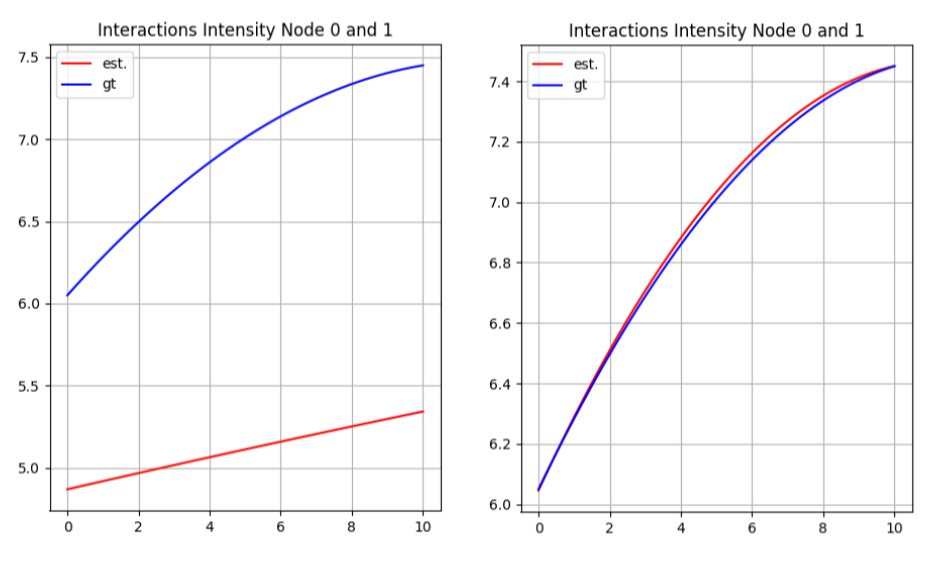
\includegraphics[width=\textwidth]{0_images/5vs5000epochs.png}
    \caption{Interaction intensity between node 0 and 1 for a given system, blue is the ground truth and red is the trained model. Left compares intensities after training the model for 5 epochs, right after training for 5000 epochs.}
    \label{fig:5vs5000epochs}
\end{figure}


\subsubsection{Node Pair Removal}
\label{sec:Method:Evaluation:NodePairRemoval}
Building on top of intensity rate comparison for node pairs, a very concrete test of modelling performance and to some extend modelling stability is devised.
For a given TDGN consisting of $N$ nodes, with a dataset consisting of interactions between $\frac{N\cdot(N-1)}{2}$ pairs of nodes (assuming they all interact), a fraction of about 10\% of the node pairs, or dyads as they may be called, are removed from the dataset before training.
After training, the modelled intensity of interaction is compared with the ground truth, revealing how well the model is able to model the TDGN with entirely missing dyads, and to some extend how well it is able to infer the interactions of removed dyads based solely on their non-removed counterparts.


\subsubsection{AUC score of removed nodes}
\label{sec:Method:Evaluation:AUC}
In order to test the model on real data, a test which does not require a ground truth model is devised.
From the dataset, 10\% of interactions are removed before training.
For each time point in the removed interactions, an alternative, false interaction is sampled, and the model is posed with evaluating the probability of the real interaction contra the false one.

The AUC score is computed as the area under the ROC (Receiver Operating Characteristics) curve.
The ROC curve is the False Positive rate vs. the True Positive rate at some given decision thresh holds.



